\documentclass{ximera}

\graphicspath{{./}{thePythagoreanTheorem/}{deMoivreSavesTheDay/}{complexNumbersFromDifferentAngles/}}

\usepackage{tikz}
\usepackage{tkz-euclide}
\usetkzobj{all}
\tikzstyle geometryDiagrams=[ultra thick,color=blue!50!black]
\newcommand{\tri}{\triangle}
\renewcommand{\l}{\ell}
\renewcommand{\P}{\mathcal{P}}
\newcommand{\R}{\mathbb{R}}
\newcommand{\Q}{\mathbb{Q}}

\newcommand{\Z}{\mathbb Z}

\renewcommand{\vec}{\mathbf}
\renewcommand{\d}{\,d}



%% Egyptian symbols

\usepackage{multido}
\newcommand{\egmil}[1]{\multido{\i=1+1}{#1}{
\includegraphics[scale=.1]{egyptian/egypt_person.pdf}\hspace{0.5mm}}}
\newcommand{\eghuntho}[1]{\multido{\i=1+1}{#1}{
\includegraphics[scale=.1]{egyptian/egypt_fish.pdf}\hspace{0.5mm}}}
\newcommand{\egtentho}[1]{\multido{\i=1+1}{#1}{
\includegraphics[scale=.1]{egyptian/egypt_finger.pdf}\hspace{0.5mm}}}
\newcommand{\egtho}[1]{\multido{\i=1+1}{#1}{
\includegraphics[scale=.1]{egyptian/egypt_lotus.pdf}\hspace{0.5mm}}}
\newcommand{\eghun}[1]{\multido{\i=1+1}{#1}{
\includegraphics[scale=.1]{egyptian/egypt_scroll.pdf}\hspace{0.5mm}}}
\newcommand{\egten}[1]{\multido{\i=1+1}{#1}{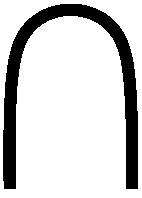
\includegraphics[scale=.1]{egyptian/egypt_heel.pdf}\hspace{0.5mm}}}
\newcommand{\egone}[1]{\multido{\i=1+1}{#1}{
\includegraphics[scale=.1]{egyptian/egypt_stroke.pdf}\hspace{0.5mm}}}
\newcommand{\egyptify}[7]{
 \multido{\i=1+1}{#1}{
\includegraphics[scale=.1]{egyptian/egypt_person.pdf}\hspace{0.5mm}}
 \multido{\i=1+1}{#2}{
\includegraphics[scale=.1]{egyptian/egypt_fish.pdf}\hspace{0.5mm}}
 \multido{\i=1+1}{#3}{
\includegraphics[scale=.1]{egyptian/egypt_finger.pdf}\hspace{0.5mm}}
 \multido{\i=1+1}{#4}{
\includegraphics[scale=.1]{egyptian/egypt_lotus.pdf}\hspace{0.5mm}}
 \multido{\i=1+1}{#5}{
\includegraphics[scale=.1]{egyptian/egypt_scroll.pdf}\hspace{0.5mm}}
 \multido{\i=1+1}{#6}{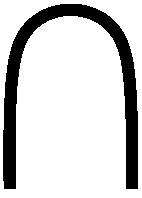
\includegraphics[scale=.1]{egyptian/egypt_heel.pdf}\hspace{0.5mm}}
 \multido{\i=1+1}{#7}{
\includegraphics[scale=.1]{egyptian/egypt_stroke.pdf}\hspace{0.5mm}}
 \hspace{.5mm}
}




\title{Leibniz and series}

\begin{document}
\begin{abstract}
In this activity we investigate some of the series that Leibniz
investigated.
\end{abstract}
\maketitle


Series pop-up at an early age. I distinctly remember being in fourth
grade, sitting at my desk, starring at my ruler, wondering how $1/3$ of
a foot could simultaneously be $4$ inches (clearly a finite number) and
$0.333333\dots$ of a foot (a number that somehow seemed finite and
infinite at the same time). I was struggling with the implicit concept that 
\[
\frac{1}{3} = \frac{3}{10}+\frac{3}{100}+\frac{3}{1000}+\frac{3}{10000}+\cdots
\]
Leibniz (and other mathematicians of the era) had similar feelings regarding series. Leibniz's mentor, Christian Huygens, suggested that Leibniz work on computing the sum of the reciprocal of the triangular numbers. Recall that the triangular numbers are the number of dots in discrete equilateral triangles:
\begin{image}
\newlength\radius
\pgfmathsetlength{\radius}{0.2cm}
\newcommand\drawballs[2][]{%
    \foreach \y [evaluate=\y as \yy using #2+1-\y] in {1,...,#2} {%
        \foreach \x in {1,...,\yy} {%
            \shade[shading=ball,ball color=white,#1] 
                ({(2*\x-2+\y)*\radius},{sqrt(3)*\y*\radius}) circle (\radius); 
        };
    }%
}
\begin{tikzpicture}
    \drawballs{1}
    \drawballs[xshift=2cm]{2}
    \drawballs[xshift=5cm]{3}
    \drawballs[xshift=8cm]{4}
\end{tikzpicture}
\end{image}

\begin{question}
Consider Leibniz's ``proof.''
\begin{align*}
S &= 1+ \frac{1}{3} + \frac{1}{6} + \frac{1}{10} + \frac{1}{15} + \frac{1}{21} + \cdots\\
\frac{S}{2}&=\frac{1}{2} + \frac{1}{6} + \frac{1}{12} + \frac{1}{20} + \frac{1}{30}+\frac{1}{42} + \cdots\\
\frac{S}{2}&=\left(1-\frac{1}{2}\right) + \left(\frac{1}{2}-\frac{1}{3}\right) + \left(\frac{1}{3}-\frac{1}{4}\right) + \left(\frac{1}{4}-\frac{1}{5}\right) + \cdots\\
\frac{S}{2}&=1+\left(-\frac{1}{2} + \frac{1}{2}\right)+\left(-\frac{1}{3} + \frac{1}{3}\right)+\left(-\frac{1}{4} + \frac{1}{4}\right)+ \cdots\\
\frac{S}{2}&= 1\\
S &= 2.
\end{align*}
Can you explain what is going on here? Where might Leibniz want to be a bit more rigorous?
\end{question}


\begin{question}
What does
\[
1-1+1-1+1-1+1-1+\cdots
\]
sum to?
\end{question}

\begin{question}
Now consider this summation of 
\[
1+ \frac{1}{3} + \frac{1}{6} + \frac{1}{10} + \frac{1}{15} + \frac{1}{21} + \cdots
\]
Write
\begin{align*}
\sum_{k=1}^\infty \frac{2}{k(k+1)} &= 1+ \frac{1}{3} + \frac{1}{6} + \frac{1}{10} + \frac{1}{15} + \frac{1}{21} + \cdots \\
\sum_{k=1}^n \frac{2}{k(k+1)} &= \sum_{k=1}^n 2\left(\frac{1}{n}- \frac{1}{n+1}\right)\\
\sum_{k=1}^n \frac{2}{k(k+1)} &= 2\left(1 - \frac{1}{n+1}\right)\\
\lim_{n\to \infty} \sum_{k=1}^n \frac{2}{k(k+1)} &= \lim_{n\to \infty}2\left(1 - \frac{1}{n+1}\right)\\
\sum_{k=1}^\infty \frac{2}{k(k+1)} &= 2.
\end{align*}
What's going on here? How does this compare to Leibniz's proof?
\end{question}

%% \begin{question}
%% Explain how the following picture ``proves'' that 
%% \[
%% 1+ \frac{1}{3} + \frac{1}{6} + \frac{1}{10} + \frac{1}{15} + \frac{1}{21} + \cdots = 2.
%% \]
%% \begin{image}
%% \begin{tikzpicture}[geometryDiagrams]
%%   \begin{axis}[
%%       domain=0:6.5,
%%       ymin=0,
%%       ymax=2.5,
%%       xmin=0,
%%       xmax=6.5,
%%       axis lines =middle, xlabel=$x$, ylabel=$y$,
%%       every axis y label/.style={at=(current axis.above origin),anchor=south},
%%       every axis x label/.style={at=(current axis.right of origin),anchor=west},
%%       axis on top,
%%     ]
%%     \addplot [draw=none, fill=blue!50!white, domain=(1:2)] {2} \closedcycle; 
%%     \addplot [draw=none, fill=white, domain=(1:2)] {1} \closedcycle; 
%%     \addplot [domain=(.5:4.3)] {2/x};
%%     \addplot [domain=(6.3:4.7)] {2/x};       
%%     %\addplot [draw=none, fill=fillp, domain=(1:2)] {1} \closedcycle;
%%     %\node at (axis cs:-.5,-.5) [textColor] {\scalebox{2}{$\boldsymbol-$}};
%%     %\node at (axis cs:2,.5) [textColor] {\scalebox{2}{$\boldsymbol+$}};
%%   \end{axis}
%% \end{tikzpicture}
%% \end{image}
%% \end{question}


In addition to (co)inventing calculus, Leibniz, dreamed up this beast
while trying to solve problems like the one posed to him by Huygens:
\[
\begin{tabular}{@{\,}c@{\,}c@{\,}c@{\,}c@{\,}c@{\,}c@{\,}c@{\,}c@{\,}c@{\,}}
& & & & $\frac{1}{1}$ & & & & \\
& & & $\frac{1}{2}$ & & $\frac{1}{2}$ & & & \\
& & $\frac{1}{3}$ & & $\frac{1}{6}$ & & $\frac{1}{3}$ & & \\
& $\frac{1}{4}$ & & $\frac{1}{12}$ & & $\frac{1}{12}$ & & $\frac{1}{4}$ &\\
$\frac{1}{5}$ & & $\frac{1}{20}$ & & $\frac{1}{30}$ & & $\frac{1}{20}$ & & $\frac{1}{5}$
\end{tabular}
\]

\begin{question} 
What relationships can you find between the entries of the triangle as
we move from row to row?
\end{question}


\begin{question} 
What are the next two rows? Clearly articulate how to produce more
rows of the harmonic triangle.
\end{question}

\begin{question} Explain how the following expression
\[
\frac{1}{r\cdot\binom{r-1}{c-1}}
\]
corresponds to entries of the harmonic triangle. Feel free to draw
diagrams and give examples.
\end{question}

\begin{question}  
Explain how the harmonic triangle is formed. In your explanation, use
the notation
\[
\frac{1}{r\cdot\binom{r-1}{c-1}}
\]
If you were so inclined to do so, could you state a single equation
that basically encapsulates your explanation above?
\end{question}

\begin{question} 
Can you explain why the numerators of the fractions in the harmonic
triangle must always be $1$?
\end{question}


\begin{question} Explain how to use the harmonic triangle to go from:
\[
\frac{1}{2} + \frac{1}{6} + \frac{1}{12} + \frac{1}{20}+\cdots
\]
to
\[
\left(1 - \frac{1}{2}\right) + \left(\frac{1}{2}-\frac{1}{3}\right) + 
\left(\frac{1}{3}- \frac{1}{4}\right) + \left(\frac{1}{4}-\frac{1}{5}\right) + \cdots 
\]
Conclude by explaining why Leibniz said:
\[
\frac{1}{2} + \frac{1}{6} + \frac{1}{12} + \frac{1}{20}+\cdots = 1
\]
\end{question}

\begin{question} 
Can you generalize the results above? Can you give a list of infinite
sums and conjecture what they will converge to?
\end{question}
\end{document}
